\documentclass[a4paper,11pt]{article}

\usepackage{microtype}
\usepackage{geometry}
\usepackage{graphicx}
\usepackage{setspace}
\usepackage{xcolor}
\usepackage{natbib}
\usepackage{float}
\usepackage{subcaption}

\usepackage[hyperindex,breaklinks]{hyperref}
% Optional customization
\hypersetup{
    colorlinks=true,
    citecolor=green,
    linkcolor=red,
    filecolor=magenta,      
    urlcolor=cyan,
}

\begin{document}

\begin{titlepage}
	\centering
	\includegraphics[width=\textwidth]{City\_logo.jpg} \\[4em]
	\begin{bfseries}
		\begin{Huge}
			Deep Learning for Image Analysis \\[35pt]
			\textsl{Written Report}
		\end{Huge}
	\end{bfseries}
	\vfill{}
	\begin{LARGE}
		\begin{sffamily}
			Martin Fixman and Grigorios Vaitsas \\[10pt]
			2023/2024 Term
		\end{sffamily}
	\end{LARGE}
\end{titlepage}

\section{Introduction}
In this study we have deployed the freely available Cityscapes dataset \cite{DBLP:journals/corr/CordtsORREBFRS16} to perform semantic segmentation analysis on urban scene imagery using a variety of Deep Learning architectures. Semantic segmentation is a computer vision technique used to identify and label specific parts of an image at pixel level. The main goal is to partition an image into areas (segments) that correspond to different objects or classes of interest (for example person, car, tree, road, building etc.). This technique is widely used in various fields like for instance, in autonomous driving, where it helps cars understand the  environment around them, as well as in medical imaging, remote sensing, and robotics. Semantic segmentation is typically performed using deep learning methods, particularly convolutional neural networks (CNNs) and their variants as well as more recent attention-based models. 
\section{Dataset}
The Cityscapes dataset is a large-scale dataset widely used for training and evaluating algorithms in the fields of computer vision, particularly for semantic understanding of urban street scenes. It features a collection of diverse urban street images from 50 different cities, collected across Germany and some neighbouring countries. The dataset includes over 5,000 fine annotations and 20,000 coarse annotations (see Figure \ref{fig:cityscapes}) of high-resolution images (2048$\times$1024 pixels). The fine annotations are detailed pixel-wise labels for 30 classes such as road, car, pedestrian, building, and traffic light. The detailed annotations are particularly valuable for our task where the goal is to assign a label to each pixel of the image. 

\begin{figure}[ht]
    \centering
    \begin{subfigure}{0.45\textwidth}
        \centering
        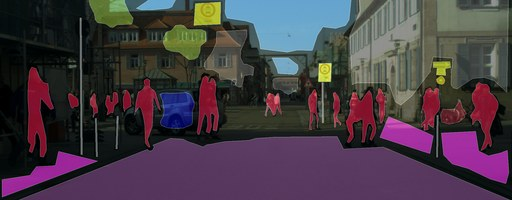
\includegraphics[width=\linewidth]{coarse_example.jpg}
        \caption{Coarse mask}
        \label{fig:sub1}
    \end{subfigure}\hfill
    \begin{subfigure}{0.45\textwidth}
        \centering
        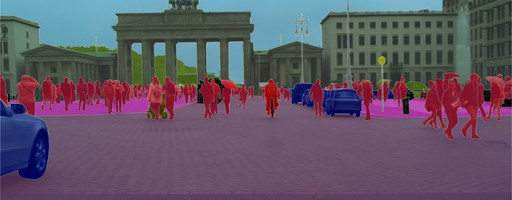
\includegraphics[width=\linewidth]{fine_example.jpg}
        \caption{Fine mask}
        \label{fig:sub2}
    \end{subfigure}
    \caption{Examples of coarse (a) and fine (b) mask annotations superimposed on the corresponding original images}
    \label{fig:cityscapes}
\end{figure}

The scenes represent a variety of seasons, daylight conditions, and weather scenarios, providing robust, real-world environments for training models that need to perform under varied conditions. This dataset has been widely used in research for developing and testing algorithms on tasks such as object detection, semantic segmentation, and instance segmentation in urban settings as well as advancing the state-of-the-art in visual perception for autonomous driving systems. The Cityscapes dataset can be accessed in the following address:
\begin{center}
\url{https://www.cityscapes-dataset.com}
\end{center}
Our particular approach in this study is to create and train at least two models; one with a basic architecture that will form our baseline and a second one where we will be exploring a more complex architecture. We are aiming to demonstrate first of all that both our models are able to perform semantic segmentation on the chosen dataset. Our second goal is to investigate how the choice of various hyper-parameters and tweaks in architecture can affect the accuracy and performance of the models. 

\section{Architectures}

Modern, state-of-the-art techniques for image analysis involve convolutional neural networks (CNNs) in their implementation. CNNs can be used to extract vital information from spatial features, which allow us to classify and segment objects in images. A type of neural network architecture designed specifically for semantic segmentation is the Fully Convolutional Network (FCN). This architecture, developed by researchers from UC Berkeley in 2014 \cite{DBLP:journals/corr/LongSD14}, has been influential in advancing the field of computer vision, particularly in tasks requiring dense prediction, like semantic segmentation. 
\begin{figure}[H]
    \centering 
    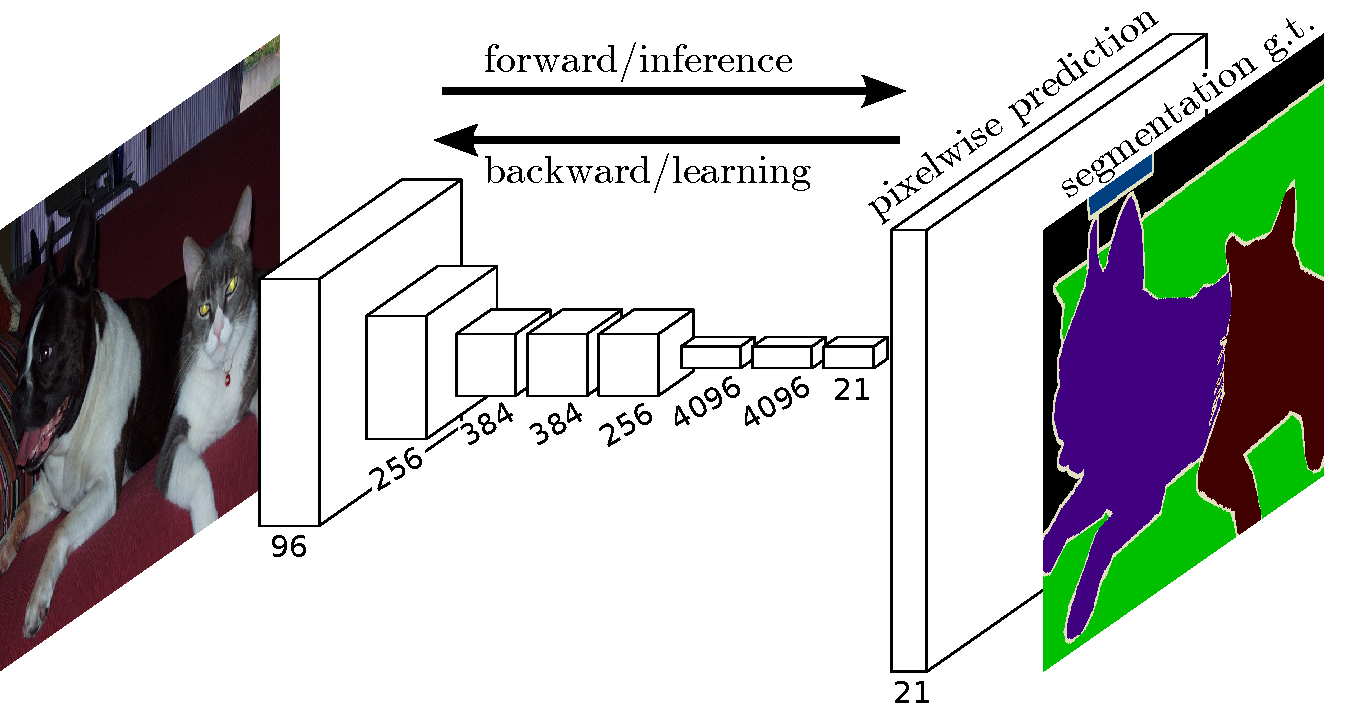
\includegraphics[width=0.7\textwidth]{alex-model.pdf}
    \caption{Example of a fully convolutional network used for semantic segmentation \cite{DBLP:journals/corr/LongSD14}}
    \label{fig:fcn-arch}
\end{figure}
Unlike standard convolutional neural networks used for image classification, which typically end with fully connected layers, FCNs are composed entirely of convolutional layers. This design allows them to take input of any size and output segmentation maps that correspond spatially to the input image, providing a per-pixel classification. FCNs transform the fully connected layers found in traditional CNNs (like those in AlexNet or VGGNet) into convolutional layers (Figure \ref{fig:fcn-arch}). This is done by treating the fully connected layers as convolutions with kernels that cover the entire input region. For example a fully connected layer that accepts an input of size 16$\times$16 can be reimagined as a convolutional layer with a 16$\times$16 filter size. To generate output segmentation maps that match the size of the input image, FCNs use transposed convolution layers (also known as deconvolutional layers) for upsampling. This process helps in recovering the spatial dimensions that are reduced during the pooling or convolutional operations in earlier layers. FCNs often utilize skip connections to combine deep, semantic information from lower layers with the shallow, appearance information in the upper layers of the network. This helps in improving the accuracy and detail of the output segmentation maps, as it allows the network to use both high-level and low-level features. 

Further improving upon the architecture of the fully convolutional network, the U-net, first introduced in a paper by Olaf Ronneberger, Philipp Fischer and Thomas Brox in 2015 \cite{DBLP:journals/corr/RonnebergerFB15}, has become very popular due to its efficiency and effectiveness, especially where data is limited. U-Net's architecture is distinctive because of its symmetric shape, which resembles the letter "U" (see Figure \ref{fig:u-netarch}). 
\begin{figure}[H]
    \centering 
    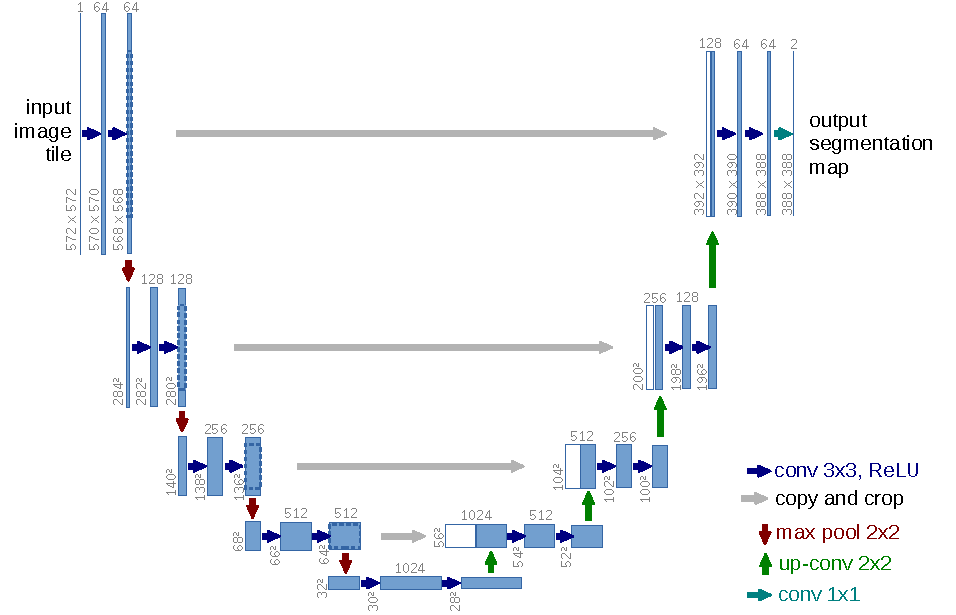
\includegraphics[width=0.7\textwidth]{u-net-illustration-correct-scale2.pdf}
    \caption{Example of the original U-net architecture as presented in \cite{DBLP:journals/corr/RonnebergerFB15}}
    \label{fig:u-netarch}
\end{figure}
It consists of two main parts: the left side of the U-net is the contracting path (encoder) which is designed to capture the context of the input image. This path is essentially a typical convolutional network that consists of repeated application of convolutions, followed by rectified linear unit (ReLU) activations, and max pooling for downsampling. Each of these steps helps in capturing the features at different levels of abstraction. On the right side of the network is the expansive path (Decoder), which performs the task of precise localization using transposed convolutions for upsampling. This part of the network gradually recovers the spatial dimensions and detail of the input image. The upsampling in the expansive path is combined with the high-resolution features from the contracting path via skip connections. These connections are crucial as they help in propagating context information to higher resolution layers, which enhances the accuracy of the output segmentation maps. U-Net's design is particularly effective in providing good segmentation results even with small training datasets, which has led to its widespread adoption and adaptation in different segmentation tasks beyond its initial medical imaging focus.

The last architecture we employed in our study was a Vision Transformer (ViT), which is a novel approach to applying transformer models, primarily used in Natural Language Processing (NLP) tasks, to image recognition. In the paper "An Image is worth 16$\times$16 Words: Transformers for Image Recognition at scale" \cite{DBLP:journals/corr/abs-2010-11929}, the authors proposed a method that treats an image as a sequence of fixed-size patches (similar to words in NLP). Each patch is embedded similarly to how tokens are embedded in NLP, and then processed by a standard transformer encoder. An overview of this model is depicted in Figure \ref{fig:vit-arch}.

\begin{figure}[H]
    \centering 
    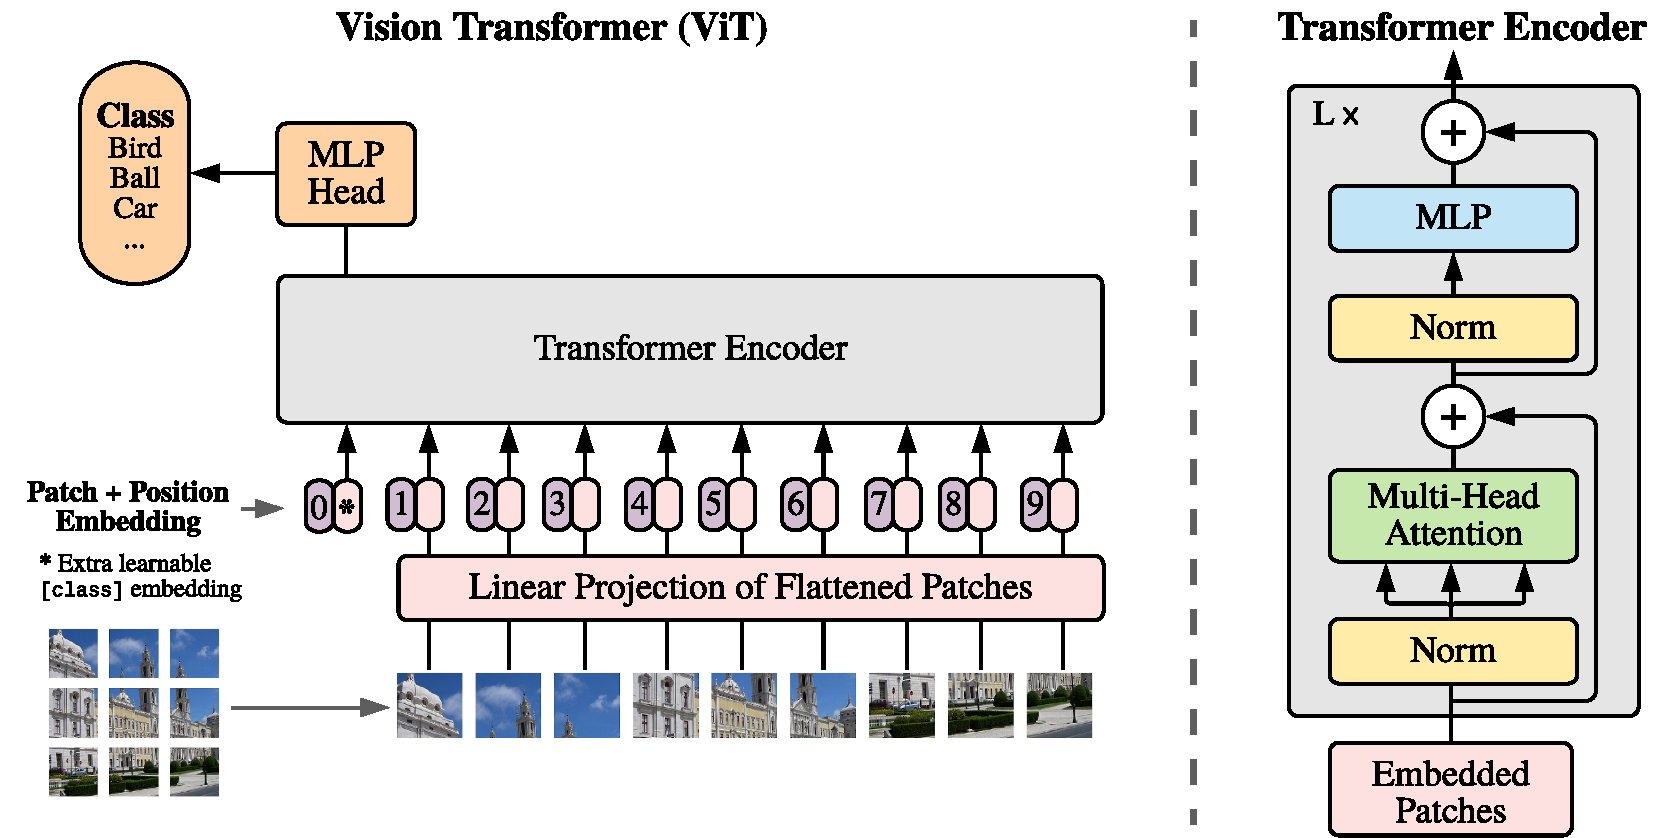
\includegraphics[width=0.8\textwidth]{model_scheme.pdf}
    \caption{Model overview of a Vision Transformer \cite{DBLP:journals/corr/RonnebergerFB15}}
    \label{fig:vit-arch}
\end{figure}

Vision transformers can achieve excellent results, outperforming many advanced CNN architectures, particularly when pre-trained on very large datasets. However, the computational complexity especially when applied on high-resolution images increases rapidly, especially for dense prediction tasks like semantic segmentation. For this reason, an improved approach has been suggested as the Swin Transformer model \cite{DBLP:journals/corr/abs-2103-14030}. In contrast to the Vision Transformer that processes the entire image at once by dividing it into fixed-size patches and applying global self-attention to all patches, the Swin transformer divides the image into smaller, non overlapping windows and applies local window-based self-attention (Figure \ref{fig:swintransform}(a)). This reduces the computational complexity because the number of interactions is limited to within a window rather than across the entire image. Additionally, the Swin transformer introduces a novel mechanism of shifting these windows in alternate layers, thus enabling cross-window connections. This helps in integrating local and global contextual information more effectively (Figure \ref{fig:swintransform}(b)). Finally, the fact that the Swin transformer starts with smaller windows and gradually merges them, reducing resolution while increasing the depth of features, enables a hierarchical architecture that processes features at multiple scales. This is beneficial for various vision tasks like object detection and segmentation, where multi-scale features are crucial. These advantages make the Swin transformer suitable as a general purpose backbone for various vision tasks. 

\begin{figure}[ht]
    \centering
    \begin{subfigure}{0.45\textwidth}
        \centering
        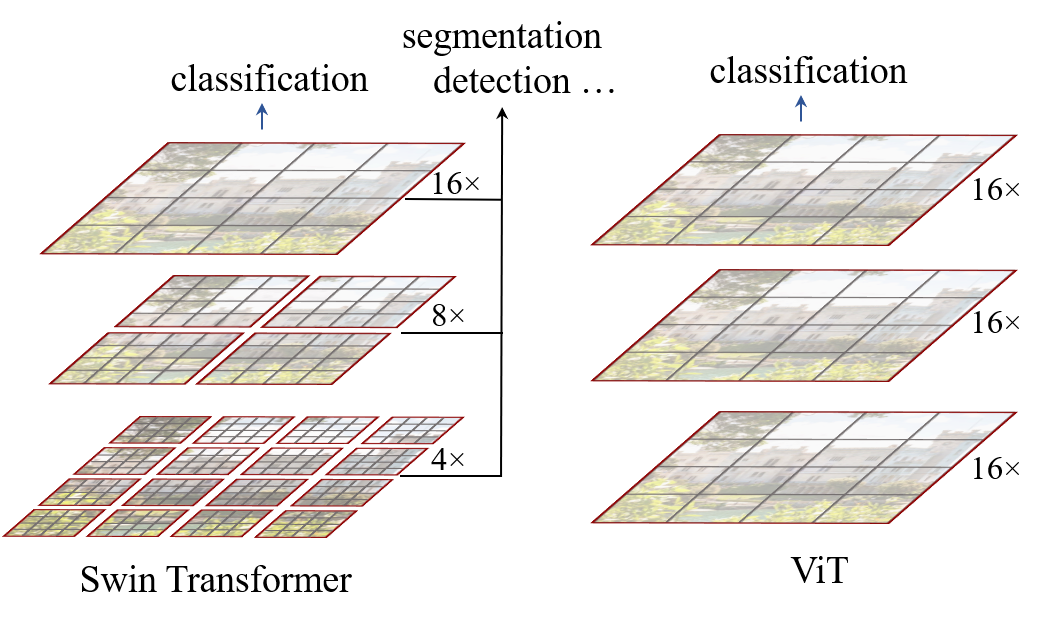
\includegraphics[width=\linewidth]{teaser11.png}
        \caption{ViT vs Swin transformer}
        \label{fig:swin-vit}
    \end{subfigure}\hfill
    \begin{subfigure}{0.45\textwidth}
        \centering
        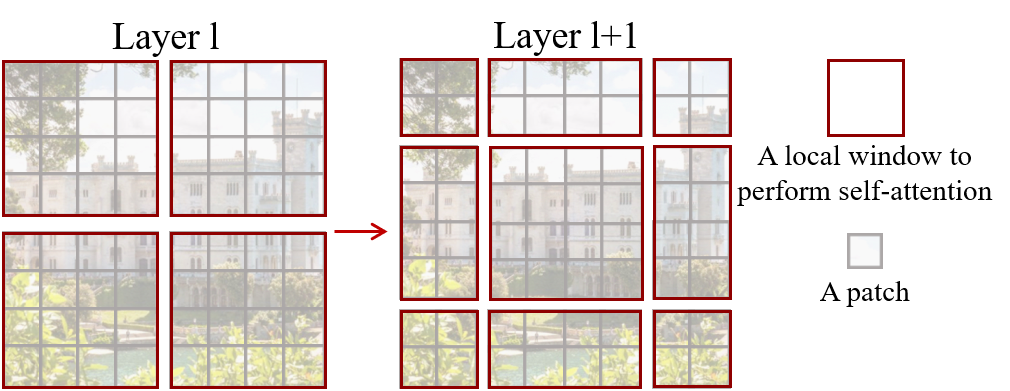
\includegraphics[width=\linewidth]{teaser_v4.png}
        \caption{The shifted window technique}
        \label{fig:shiftwindow}
    \end{subfigure}
    \caption{Characteristics of the Swin transformer\cite{DBLP:journals/corr/abs-2103-14030}}
    \label{fig:swintransform}
\end{figure}

\section{Methodology}

\section{Results}

\section{Conclusions}

\section{Reflections}

\bibliographystyle{plain}
\bibliography{convolutional_assessment}


\end{document}
